\documentclass[../../ASSD_TP1_G7.tex]{subfiles}
\begin{document}
\chapter*{Oscilador}
Se dise\~no un oscilador cuya salida sea cuadrada, de frecuencia variable y de duty cycle variable. Ambos parámetros capases de variar independientemente uno de otro.
\subsection*{Circuito implementado}
Para lograr la independencia en la variación de frecuencia y duty cycle, se propuso un circuito de dos bloques, uno encargado de la frecuencia y el otro del duty cycle.
\begin{figure}[H]
\centering
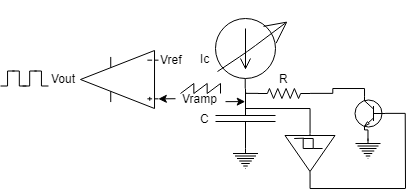
\includegraphics[width=0.5\textwidth]{figures/diagBloques.png}
\caption{Diagrama en bloques del circuito}
\end{figure}
\par El bloque correspondiente al control de la frecuencia es el de la fuente variable de corriente, el capacitor y el schmitt trigger. Como $i_c=\frac{d_v}{d_t}$, donde $i_c$ es la corriente en el capacitor, es constante debido a la fuente de corriente entonces la tension en el capacitor crece lienealmente en el tiempo,$V_c=t \frac{i_c}{C}$. Alcanzado la tension $V_{high}$ del schmitt trigger, su salida pasara a nivel alto y el transistor entrara en saturacion, descargando el capacitor. Cuando la tension el el capacitor alcance la tension $V_{low}$, la salida del schmitt trigger pasara a nivel bajo y la descarga del capacitor se detiene.
Variando $i_c$ se generan distintas pendientes de la rampa, a mayor pendiente mayor frecuencia. 
\par El bloque correspondiente al control del duty cycle, es el del comparador. Variando la tension de referencia($V_{ref} $), del comparador se logra el control del duty cycle. Cuando la tension en el capacitor supera a $V_{ref} $ la salida del comparador pasa a estado alto.
\subsubsection*{Implementación del modulo de control de frecuencia}
El modulo consta de dos partes:
\begin{itemize}
  \item Fuente variable de corriente
  \item Modulo para descargar el capacitor
\end{itemize}

La fuente de corriente implementada es la de la figura \ref{fig:fuenteCorriente}. 
\begin{figure}[H]
\centering
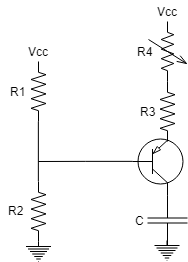
\includegraphics[width=0.25\textwidth]{figures/fCorriente.png}
\caption{Fuente de corriente implementada}\label{fig:fuenteCorriente}
\end{figure}
Recorriendo la malla de entrada se obtiene la siguiente ecuación para la corriente de base del transistor
\begin{equation}
i_b=\frac{V_{cc}-V_{cc}\frac{R_2}{R_1 + R_2}-V_{be}}{(\beta + 1)(R_3 + R_4)}
\end{equation}
Sabiendo que $i_c=\beta i_b$ entonces:
\begin{equation}
i_c= \frac{\beta}{\beta + 1} \left( V_{cc} \frac{R_1}{R_1 + R_2} -V_{be} \right) \frac{1}{(R_3 + R_4)} \label{eq:ic}
\end{equation}
Llamando 
\begin{equation}
K=\frac{\beta}{\beta + 1} \left( V_{cc} \frac{R_1}{R_1 + R_2} -V_{be} \right)
\end{equation}
Reemplazando $K$ en \ref{eq:ic}:
\begin{equation}
i_c=\frac{K}{R_3 + R_4} \label{eq:icfin}
\end{equation}

Como la corriente en el capacitor es constante entonces
\begin{equation}
V_c=i_c t \label{eq:vc}
\end{equation}

Reemplazando la ecuación \ref{eq:icfin} en \ref{eq:vc} se obtiene la expresión final
\begin{equation}
V_c=\frac{K}{R_3 + R_4} t 
\end{equation}

\par El modulo encargado de la descarga del capacitor, se implemento con un LM555, debido a que en un mismo integrado se encuentra el schmitt trigger y el transistor. \todo{no me gusta la gustificacion}
\begin{figure}[H]
\centering
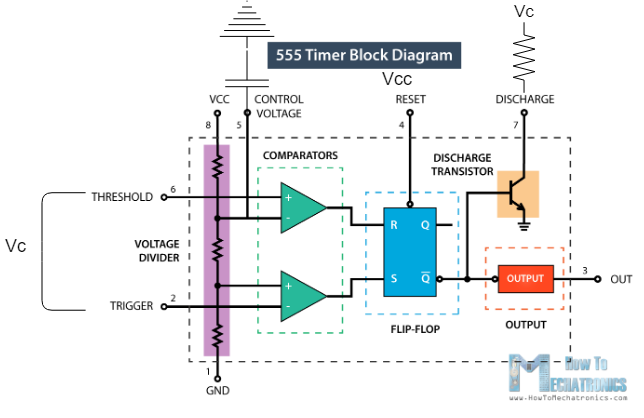
\includegraphics[width=0.6\textwidth]{figures/descargaC.png}
\caption{Modulo encargado de la descarga del capacitor}\label{fig:descargac}
\end{figure}

Al juntar  el pin de TRESHOLD y TRIGGER del LM555 se consigue que este se comporte de la siguiente manera

\begin{table}[htbp]
\begin{center}
\begin{tabular}{|l|l|}
\hline
$V_c$ & $\bar{Q_n}$ \\
\hline \hline
$V_c>\frac{2}{3}V_{cc}$ & 1 \\ \hline
$\frac{1}{3}V_{cc}<V_c<\frac{2}{3}V_{cc}$ & $\bar{Q_{n-1}}$ \\ \hline
$\frac{1}{3}V_{cc}<V_c$ & 0 \\ \hline
\end{tabular}
\caption{Comportamiento del circuito}

\end{center}
\end{table}
El comportamiento indicado en la tabla corresponde al de un schmitt trigger.

\par Juntando ambos módulos ya mencionados se obtiene un circuito que genera un diente de cierra a frecuencia variable dependiendo de a tension de entrada y de la resistencia variable.
\par Finalmente a partir de las ecuaciones previamente desarrolladas y de los niveles de tension $V_{high}$ y $V_{low}$ se obtuvo la expresión de la frecuencia del circuito:

\begin{equation}
f=\frac{K}{\frac{1}{3}V_{cc} (R_3+R_4) C}
\end{equation}

\subsubsection*{Implementación del modulo de control de duty cicle}
\par El núcleo de este modulo es un comparador, en este caso se utilizo un LM311. La salida del comparador es open collector, por ende hay que incluir en el circuito una resistencia de pull up.
\par 

\begin{figure}[H]
\centering
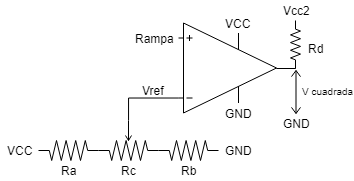
\includegraphics[width=0.4\textwidth]{figures/comp.png}
\caption{Circuito del modulo de control de duty cicle}\label{fig:comp}
\end{figure}
El objetivo de las resistencias $R_b$ $R_c$ y $R_d$, es generar una tension de referencia para el comparador.
\begin{equation}
V_{ref}=Vcc \frac{R_ck + Rb}{R_a + R_c + R_b}
\end{equation}
Donde $k$ es una constante cuyo valor varia entre 0 y 1, representando la posición del preset. El objetivo de las impedancias $R_a$ y $R_b$ es limitar el valor máximo y mínimo de $V_{ref}$. 

\begin{figure}[H]
\centering
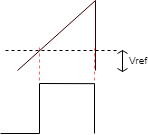
\includegraphics[width=0.3\textwidth]{figures/r2sq.png}
\caption{Ejemplo de funcionamiento}\label{fig:ej}
\end{figure}

La figura \ref{fig:ej}, muestra el funcionamiento del comparador para variar el duty cycle. Si $V_{ref}$ aumenta el tiempo el tiempo que la se\~al se encuentra en el nivel bajo, es decir el duty cycle disminuye. Entonces variando la $V_{ref}$ se logra controla del duty cycle. 
\par Conociendo la tension máxima de la rampa se puede hallar la formula del duty cycle($DC$):
\begin{equation}
DC=\left[ 1 - \frac{Vcc \frac{R_ck + Rb}{R_a + R_c + R_b}}{V_{max}} \right] 100
\end{equation}

\subsection*{Características del oscilador}
El oscilador posee las siguientes carcateristicas:
\begin{itemize}
  \item Frecuencia máxima $300KHz$
  \item Frecuencia mínima $1KHz$
  \item Duty cycle mínimo 4\%
  \item Duty cycle máximo 98\%
  \item $v_o$ mínimo -15v
  \item $v_o$ máximo 15v

\end{itemize}
Se midió el la salida del generador:

\begin{figure}[H]
\centering
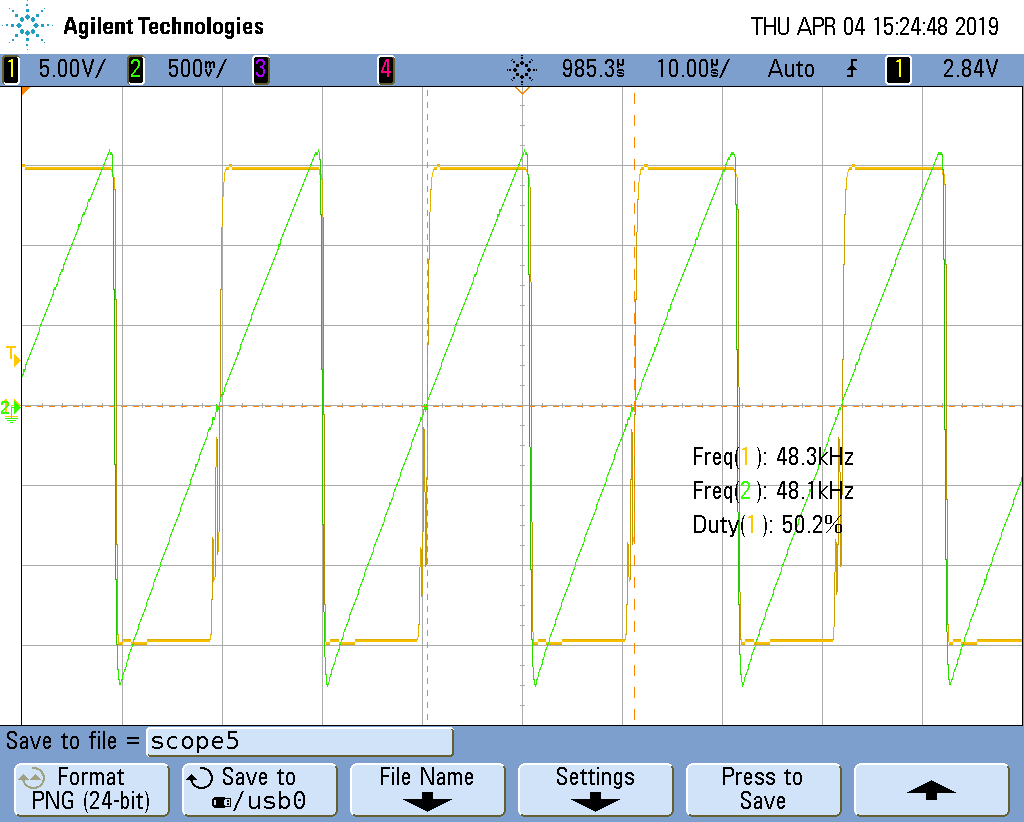
\includegraphics[width=0.4\textwidth]{figures/scope5.png}
\caption{Frecuencia de 50KHz y duty cycle 50\%. Se\~nal verde tension en el capacitor, la amarilla salida del comparador}
\end{figure}

\begin{figure}[H]
\centering
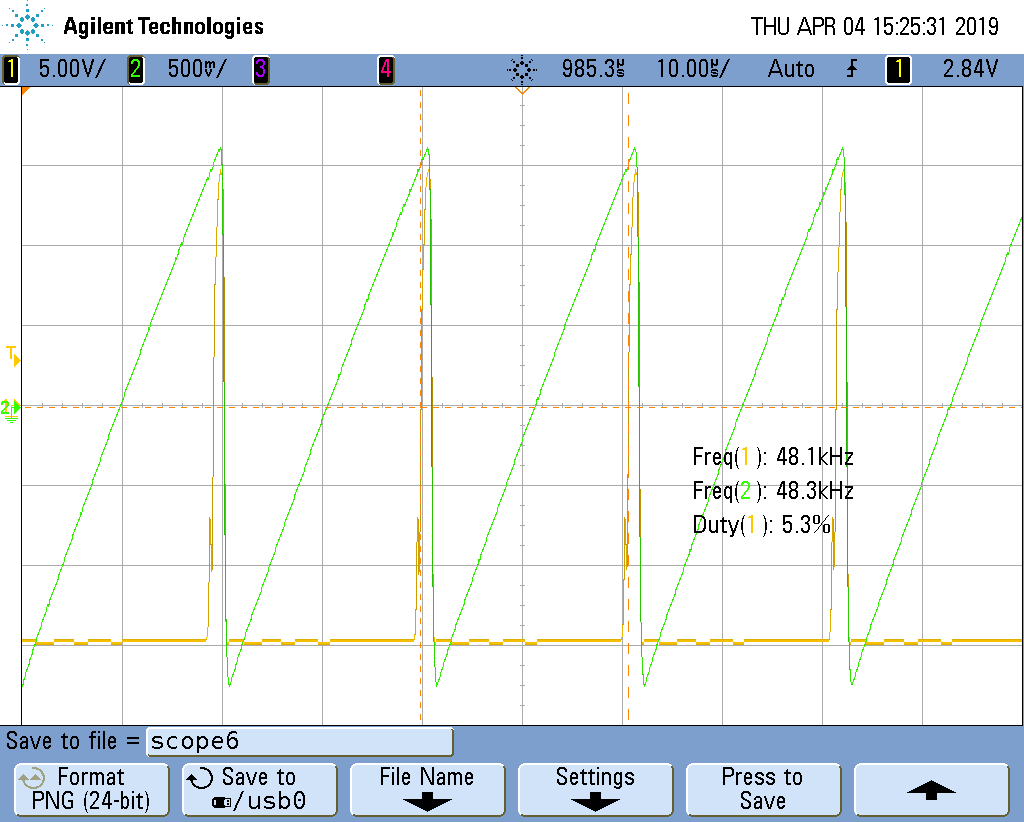
\includegraphics[width=0.4\textwidth]{figures/scope6.png}
\caption{Frecuencia de 50KHz y duty cycle 5\%. Se\~nal verde tension en el capacitor, la amarilla salida del comparador}
\end{figure}

\begin{figure}[H]
\centering
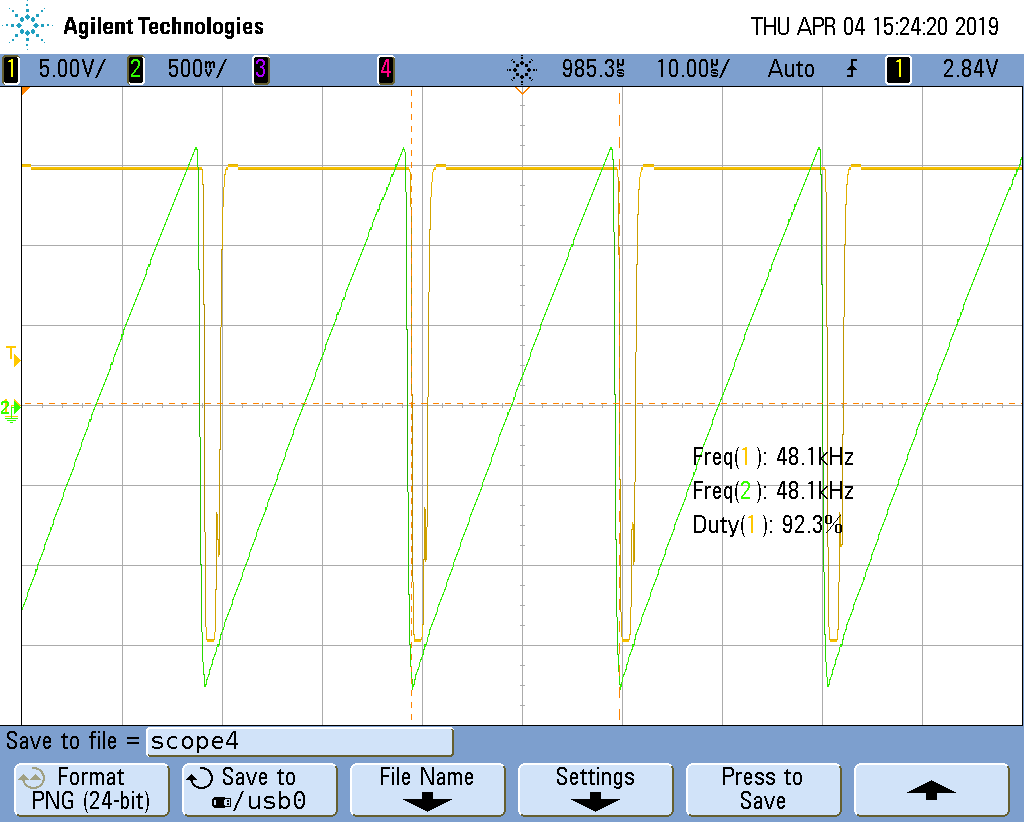
\includegraphics[width=0.4\textwidth]{figures/scope4.png}
\caption{Frecuencia de 50KHz y duty cycle 92\%. Se\~nal verde tension en el capacitor, la amarilla salida del comparador}
\end{figure}





\subsection*{Consideraciones al utilizar se\~nales analógicas y digitales en un mismo circuito }
\par En los circuitos donde hay se\~nales analógicas y digitales mezcladas hay que tener especial consideración en la influencia de las se\~nales digitales en las analógicas. Esto se debe a que en los circuitos digitales existen umbrales para discernir el estado de una se\~nal. 
\par Los principales efectos que se pueden manifestar son\footnote{Grounding in mixed-signal systems demystified, Part 1. (2019). [ebook] Disponible en: http://www.ti.com/lit/an/slyt499/slyt499.pdf [Accedido 23 Mar. 2019].}:
\begin{itemize}
  \item Perdida de referencia a tierra 
  \item Se\~nales que se copian a otras pistas 

\end{itemize}

\par El fenómeno de la copia de se\~nales a pistas cercanas, se debe a las capacidades parásitas entre las pistas. Para evitarlo entre dichas  pistas tiene que haber una pista con masa.
\subsubsection*{Perdida de referencia a tierra}
 En circuitos donde hallan se\~nales cuadradas, en el momento del flanco positivo de la señal se produce un pico de corriente, uno de los posibles caminos por donde la corriente vuelve a la fuente es por tierra. Supongamos que en una misma pista tiene conectada la tierra de un comparador y la referencia a cero volt de un circuito analógico. En el momento que la salida del comparador pasa de estado bajo a alto se produce un pico de corriente, y la resistencia considerada despreciable en la pista de masa deja de serlo, entonces se produce una caída de tension sobre esa pista y la referencia del circuito analógico se pierde. 
 \par Dos posibles opciones para minimizar este efecto son
 \footnote{Grounding in mixed-signal systems demystified, Part 2. (2019). [ebook] Disponible en: http://www.ti.com/lit/an/slyt512/slyt512.pdf [Accedido 23 Mar. 2019].}:
 \begin{itemize}
  \item Pistas gruesas y cortas
  \item Planos de masa 
\end{itemize}
Ambas soluciones implican separar las masas de los circuitos analógicos de los digitales.
En vez de tener un único plano de masa para toda la placa, separarlo en plano de masa para el circuito digital y para el circuito analógico, y unirlos en un único punto. También se pueden agregar inductores entre los planos de masa, permitiendo que las bajas frecuencias pasen y las altas no.
\par Otra solución posible es utilizar una topologia estrella para la coneccion de las masas (todas a un mismo punto), esta solucion dificulta el ruteo. Una variación de este método es no conectar por separado las masas del circuito analógico del digital y usar pistas anchas. De esta manera se reduce la impedancia de las pistas, minimizando la caída de tension en ella.









\end{document}
